%%% Local Variables:
%%% mode: latex
%%% TeX-master: "../doc"
%%% coding: utf-8
%%% End:
% !TEX TS-program = pdflatexmk
% !TEX encoding = UTF-8 Unicode
% !TEX root = ../doc.tex
Das entwickelte Tool, \e{lode}, ist ein erster Schritt in die Richtung einer \e{LOD}-Pipeline, welche für das Web optimiert wurde. Das Tool erreicht das Ziel, für eine Vielzahl von Anwendungsgebieten einsetzbar zu sein. Wichtig ist es jedoch festzuhalten, dass es nicht für alle Anwendungen angemessen ist. Zum einen soll die Pipeline weiter entwickelt und in ihren Kernkompetenzen gestärkt werden, zum anderen gibt es jedoch auch spezifische Gebiete, wie zum Beispiel \e{Terrain}, für welche \e{lode} ungeeignet ist.

\section{LOD System}

Der grösste Nutzen entsteht in Anwendungen mit komplexen Modellen – für diese Situationen bietet \e{lode} einen nachweisbaren Mehrwert. Die Zahlen aus \autoref{chap:benchmarkResults} zeigen den möglichen Nutzen in einem Anwendungsbeispiel.

Die Resultate zeigen einen klaren Unterschied zwischen der unoptimierten und optimierten Version. Die \e{FPS} geben eine klare Auskunft. Unter Berücksichtigung des berechneten Konfidenzintervalls wird das Resultat als signifikant erachtet. Diese These wird auch durch eine Kontrolle mit dem Auge belegt – die Anzahl \e{FPS} unterscheidet sich merkbar. Die Ladezeit der Applikation wurde nur marginal tangiert, die Auswirkungen auf die \e{User Experience} sind vernachlässigbar und können im optimalen Fall sogar durch progressives Laden zu einem Vorteil werden.

Somit ist es möglich, einen Nutzen für bestimmte anspruchsvolle 3D-Visualisierungen zu generieren.

\subsection{Allgemeingültigkeit}

Innerhalb der Testapplikation, wie in \autoref{chap:testApplication} beschrieben, werden dieselben Modelle mehrfach angezeigt. Dies wird in der Praxis insbesondere bei repetitiven Elementen, wie zum Beispiel Bäumen für Landschaftsgestaltung, verwendet. In solchen Situationen stellen die Anzahl Polygone das primäre Problem für eine gute Laufzeitleistung dar und der Einsatz von \e{LOD}-Artefakten kann erwägt werden. Die Allgemeingültigkeit ist für Anwendungsfälle mit vergleichbaren Anforderungen gegeben.

\subsection{Anwendbarkeit}

Der in dieser Arbeit implementierte Algorithmus kann für eine Vielzahl von verschiedenen Modellen angewendet werden und liefert solide Resultate. Die geometrische Approximation ist ausreichend für ein \e{LOD}-System. Für Spezialfälle wie Randbehandlung sind entsprechende Kontrollen implementiert worden.

\subsection{Abgrenzung}

In einigen Anwendungsgebieten bringt ein \e{LOD}-System nicht den gewünschten Nutzen. Wird ein Modell nur auf einer Detailstufe angezeigt, so ist der Einsatz von \e{LOD} abzuraten. Sind die Modelle bereits sehr simpel, wie bei \e{Low-Poly}-Modellen – in Abbildung \ref{fig:lowPolyExample} zu sehen – sind die zusätzlichen Vereinfachungen nur von geringem Nutzen. Denn die Geometrie dieser Art von Modelle ist bereits sehr simpel und eine weitere Vereinfachung nur von geringer Auswirkung. Ein Beispiel eines vereinfachten Modells ist in Abbildung \ref{fig:lodModelSimplified} veranschaulicht und ähnelt stark einem \e{Low-Poly}-Modell.
So muss der Einsatz von \e{LOD}-Artefakten für jeden Anwendungsfall separat abgewogen werden. Ein Vorteil von \e{lode} ist die Einfachheit der Integration. So ist es möglich, mit wenig Aufwand den groben Nutzen für ein spezifisches Anwendungsbeispiel abschätzen zu können, ohne dass viel Entwicklungszeit dafür aufgewendet werden muss.

\begin{figure}[H]
  \begin{subfigure}{.5\textwidth}
    \centering
    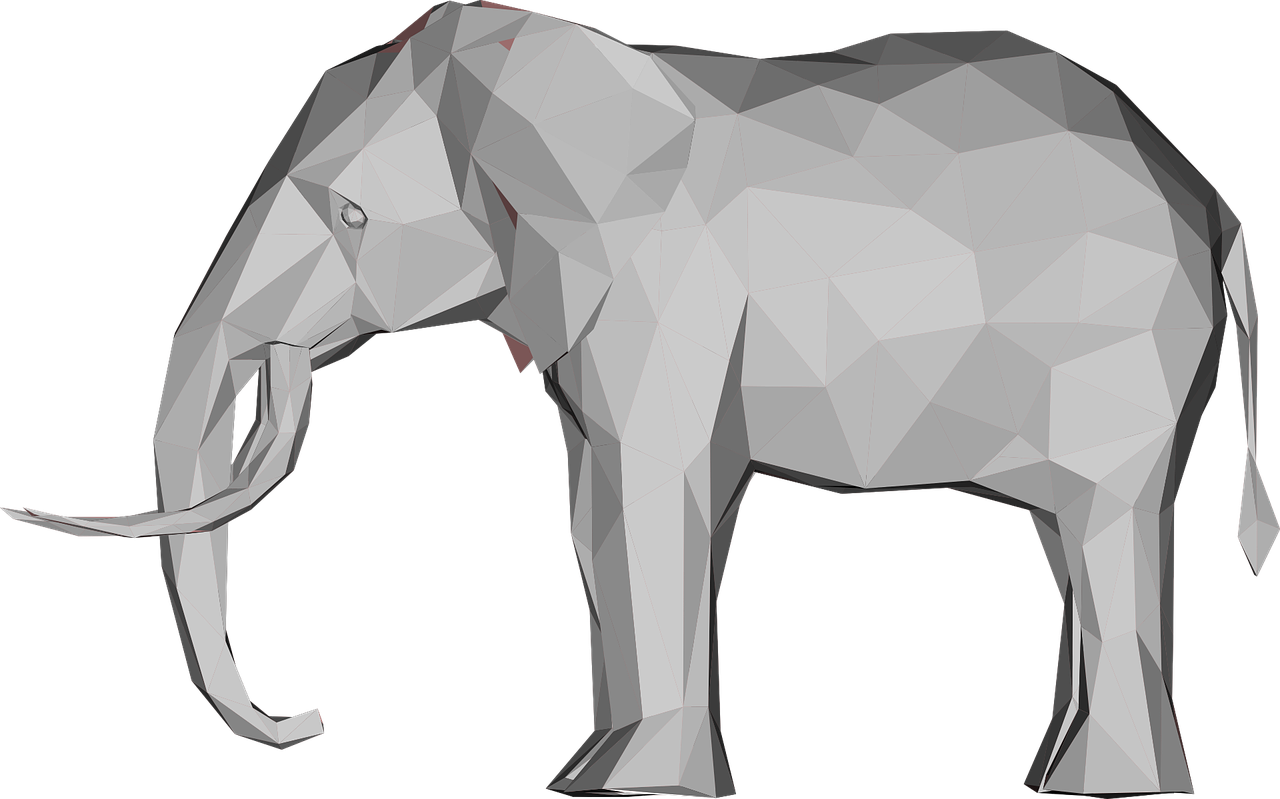
\includegraphics[width=0.4\columnwidth]{diskussion/low-poly-example.png}
    \caption{Beispiel \e{Low-Poly}-Modell}
    \label{fig:lowPolyExample}
  \end{subfigure}%
  \begin{subfigure}{.5\textwidth}
    \centering
    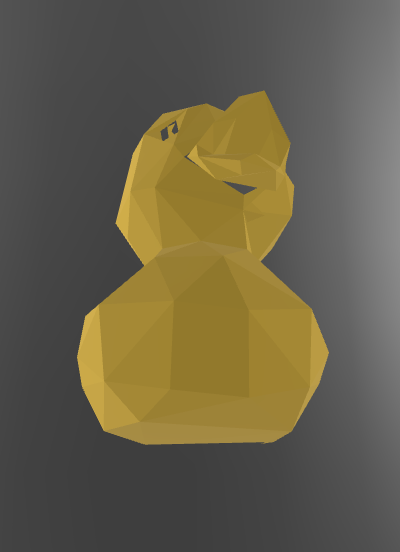
\includegraphics[width=0.4\columnwidth]{resultate/lod-simplified.png}
    \caption{Beispiel Resultat nach \e{LOD}-Simplifizierung}
    \label{fig:lodModelSimplified}
  \end{subfigure}
  \caption{Vergleich zwischen Low-Poly und \e{LOD}-simplifiziertem Model}
  \label{fig:comparisonLowPolyAndLOD}
\end{figure}

\section{Mögliche Erweiterungen}
Die Möglichkeiten für Erweiterungen zu \e{lode} sind sehr umfangreich. In diesem Abschnitt wird auf einige Möglichkeiten eingegangen.

\paragraph{Akurate Texturinformationen}
Zurzeit wird die Textur komplett entfernt und durch eine einfache Farbinformation ersetzt. Dies stellt beim aktuellen Einsatz der \e{LOD}-Artefakten kein Problem dar. Eine interessante Erweiterung ist so jedoch nicht möglich: das Vereinfachen der ersten Stufe. Der Algorithmus kann so erweitert werden, dass die Texturinformationen nicht vereinfacht, sondern als Teil der \e{Vertices} verwendet werden. Dies würde es ermöglichen, ein Modell, welches über mehrere Millionen Polygone verfügt, und somit ungeeignet für das Web ist, zu vereinfachen und diese erste Vereinfachung als detailreichste Stufe zu verwenden.

\paragraph{glTF LOD Format}
Es gibt einen Vorschlag, um die Definition von \e{LOD}-Stufen innerhalb von glTF zu definieren. Dies würde es ermöglichen, verschiedene \e{LOD}-Artefakte in einer Datei zu speichern \cite{glTFExtensionLOD}. Was wiederum erlauben würde, Texturinformationen einfacher wiederzuverwenden. Die Pipeline kann grundsätzlich für diesen Anwendungsfall erweitert werden.
Zurzeit hat Three.js jedoch noch keinen Support für diese Erweiterung. Auch Babylon.js unterstützt lediglich das progressive Laden von Modellen \cite{babylonProgressiveLoading}.

\paragraph{Progressives Laden}
Aktuell werden initial alle \e{LOD}-Artefakte geladen. Dies hat zur Konsequenz, dass im Vergleich zur unoptimierten Variante eine schlechtere initiale Ladezeit resultiert. Um dieses Verhalten zu verbessern beziehungsweise sogar in einen Vorteil zu verwandeln, könnte das System so erweitert werden, dass die Modelle progressiv geladen werden. Es würde also zuerst die kleinste Datei geladen und bereits angezeigt werden, während in der Zwischenzeit die detailreicheren Modelle nachgeladen werden und die detailärmeren ersetzen. Somit reduziert sich die Zeit bis zum ersten visuellen Feedback und die \e{User Experience} kann damit verbessert werden.

\paragraph{Levelwahl während Laufzeit}
Die optimale Wahl des Levels kann stark von der Laufzeitumgebung abhängig sein. So sollte zum Beispiel auf mobilen Geräten früher ein einfacheres Modell angezeigt werden als auf leistungsstarken Geräten. Ein weiterer Faktor ist die Auflösung. Bei Geräten mit niedriger Auflösung kann früher gewechselt werden, da die visuellen Unterschiede zum Original weniger auffällig sind.
Deshalb eignet sich eine Wahl der Levels zur Laufzeit, um ein optimales Erlebnis auf allen Geräten zu ermöglichen.
Nebst dem \e{\gls{CLI}} soll folglich auch ein Javascript-Modul bereitgestellt werden, welches das Laden von glTF Dateien übernimmt und basierend auf der erkannten Performanz das beste Level of Detail einspielt.

\paragraph{Kombination mehrerer Meshes}
Als Erweiterung ist es möglich, verschiedene \e{Meshes} eines glTF zu kombinieren und als ein einziges \e{Mesh} zu behandeln. Dies erlaubt es noch mehr Vereinfachungen vornehmen zu können. Diese Anpassung kann man als simples \e{HLOD}-System bezeichnen. Eine Schwierigkeit ist hier jedoch die sinnvolle Wahl der Textur, da vereschiedene \e{Meshes} häufig über verschiedene Texturen verfügen und diese ebenfalls kombiniert werden müssten.

\paragraph{Fading}
\label{chap:fading}
Aktuell finden die Modellwechsel an harten Grenzen statt. Dies hat zur Konsequenz, dass \e{Visual Popping} auftauchen kann. Eine Möglichkeit zur Linderung dieses Problems ist der Einsatz von \e{Fading}. Hierbei werden die Übergänge über grössere Intervalle durchgeführt und Teile der verschiedenen Artefakte dargestellt. Diese Methode wird zum Beispiel bei \e{Unity} angeboten.

\paragraph{Konsequenter Einsatz von glb Dateien}
Aktuell werden in der Demoszenerie glTF Dateien eingesetzt. Dies kommt daher, dass die Basisinformationen menschenlesbar abgespeichert werden. Das binäre Format glb ist jedoch grundsätzlich glTF vorzuziehen und sollte als primäres Austauschformat verwendet werden. Für das Laufzeitverhalten entsteht kein signifikanter Unterschied durch den Einsatz von glb. Der primäre Vorteil vom glb Format ist, dass alles in einer Datei gespeichert ist und somit nicht zwei Netzwerkabfragen stattfinden müssen – die Download\-zeit wird somit reduziert. Das CLI könnte erweitert werden, auch glb Dateien zu unterstützen.
